\section{Future Developments}

The Heat Orchestration Template (or \textsc{Hot}) format is an effort to develop a native template language for Heat.\footnote{Note that support for the CloudFormation template format will be maintained indefinitely.} A number of cosmetic changes have been prototyped already, with the aim of taking advantage of a \textsc{Yaml}-native format to improve the readability of templates.

\begin{figure*}[t]
\centering
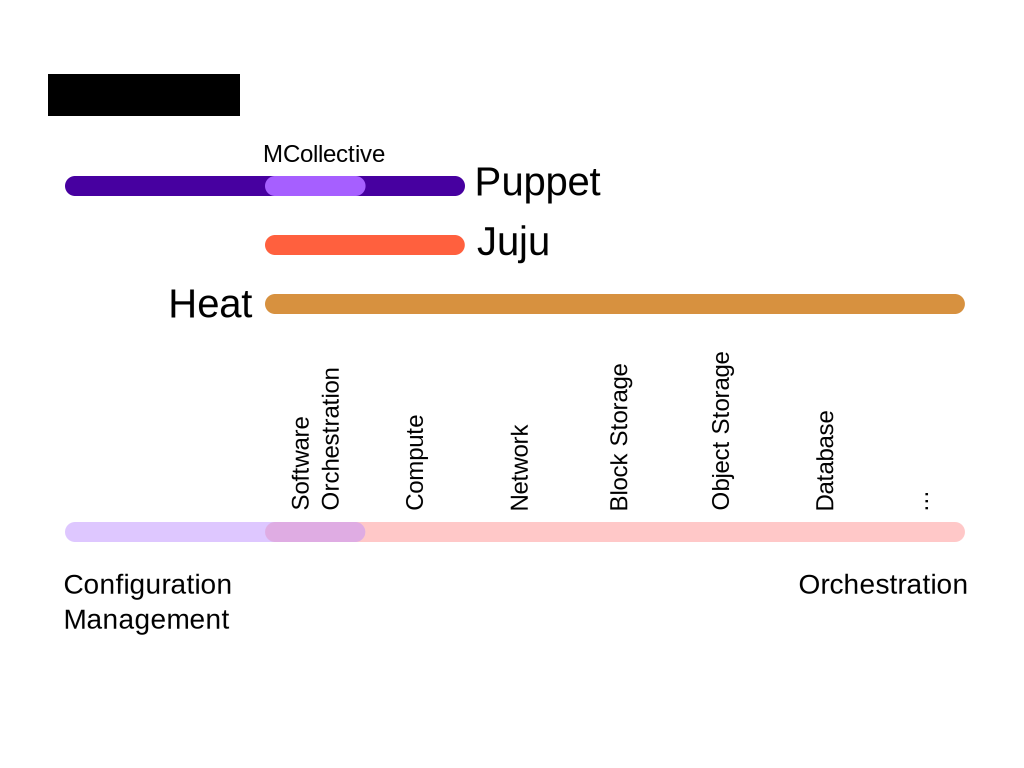
\includegraphics[trim=0em 10em 0em 17em,width=0.85\textwidth]{orchestration-config-management.pdf}
\caption{The relative positioning of Heat compared with other categories of software: configuration management systems (such as Puppet or Chef) and configuration managment--orchestration hybrids (such as Juju).}
\label{fig:orchestration-config-management}
\end{figure*}

Work on \textsc{Hot} will continue in the upcoming Icehouse development cycle to close the gap (illustrated in Figure~\ref{fig:orchestration-config-management}) between orchestration and configuration managment, which are complementary technologies.\footnote{The Heat team is working very hard to avoid any \emph{overlap} with configuration management, or reliance on any particular tool.} Likely changes involve handling dependencies and passing data between software components installed on the virtual servers that Heat configures. This will enable Heat to handle far more complex application topologies than are currently feasible.

\newthought{Development is also} planned on a separate Autoscaling API, to allow access to autoscaling for users who are not using Heat templates. We expect it to gain many more capabilities in the process, such as rolling updates and the ability to scale whole templates.
